%\documentclass[overheadsbeamer.tex]{subfiles}
\documentclass[handoutsbeamer.tex]{subfiles}

\begin{document}

\ona{ \setcounter{chapter}{10} } % ONE LESS
\lecture{Algorithmic Quantum State Tomography and Quantum Channel Tomography}{Lect11}
\chapter{Algorithmic Quantum State Tomography and Quantum Channel Tomography}\label{C.AlgTomography}

\begin{frame}\ft{Outline}
\ona{\Chaps~\ref{C.StateSpace}--\ref{C.SampleComplexity} asked \emph{whether} a quantum system can be identified from measurement data, and \emph{how much} data is needed. This \chap{} is about \emph{how}: the algorithms that turn measurement records into a density operator (state tomography), into a channel (process tomography), and finally into the parameters of a master equation (system identification proper). We move from the static problem---one unknown state, many copies---to the dynamical one, where the unknown is the generator of the evolution and the data are time series of expectation values. The pipeline is: prepare, evolve, measure; estimate states or expectation values; fit a linear dynamical system; reconstruct the Hamiltonian and Kossakowski matrix from the fitted system matrix.}
\onp{Outline of today's lecture:
\begin{itemize}\setlength\itemsep{0.6em}
    \item the pipeline: tomography $\to$ system identification $\to$ parameter reconstruction;
    \item state tomography: linear inversion, maximum likelihood, projected least squares, compressed sensing, classical shadows;
    \item process tomography: standard, ancilla-assisted, noisy circuits, gate set tomography;
    \item open-system identification from time series: ERA, Koopman, learning-based, polynomial optimization;
    \item recovery of master-equation parameters from the system matrix (Algorithms~\ref{alg:ch11:general}--\ref{alg:ch11:symmetric});
    \item Hamiltonian identification as polynomial optimization.
\end{itemize}}
\ona{\medskip\noindent\textit{Sources.} This \chap{} draws on \citep{parvaiz2026survey,parvaiz2025identifiability,bondar2025globally}; passages from these papers are reproduced with light editing.}
\onp{\vfill{\scriptsize Sources: \citep{parvaiz2026survey,parvaiz2025identifiability,bondar2025globally}.}}
\end{frame}

\section{The pipeline}

\begin{frame}\ft{From measurement records to master equations}
\ona{Most quantum system identification methods share a common structure. First, states along the trajectory $\rho(t_j)$, or at least expectation values $\langle O_i(t_j)\rangle$ of a fixed set of observables, are estimated from repeated measurements; this is (partial) quantum state tomography and is the front end of everything that follows. Second, the estimates are fitted by a dynamical model. For an autonomous GKSL system the coherence vector $x_j=\Tr(F_j\rho)$ obeys the linear dynamical system $\dot x=\bA x+\vec\beta$ of \Chap~\ref{C.Open}, so classical realisation theory applies; under control the system is bilinear. Third, the fitted system matrix $\bA$ is mapped back to the Hamiltonian coefficients $\vec\theta$ and the Kossakowski matrix $\gamma$. Each stage has its own algorithmic questions and its own failure modes: statistical noise in the first, non-uniqueness of realisations in the second, conditioning of a linear inverse problem in the third.}
\onp{\begin{enumerate}\setlength\itemsep{0.5em}
    \item \alert{Tomography}: estimate $\rho(t_j)$ or $\langle O_i(t_j)\rangle$ from shots.
    \item \alert{Identification}: fit $\dot x=\bA x+\vec\beta$ (autonomous) or $\dot x = (\bA+\sum_k u_k\mathbf B_k)x+\vec\beta$ (controlled) to the estimates.
    \item \alert{Reconstruction}: invert the map $(\vec\theta,\gamma)\mapsto(\bA,\vec\beta)$.
\end{enumerate}
Failure modes: shot noise; non-unique realisations (similarity, branches of $\log$); conditioning of $\bM$.}
\end{frame}

\begin{frame}\ft{Why not just do full tomography?}
\ona{Efficient algorithms, in terms of both the sample and classical post processing complexity, have been developed for quantum state tomography (QST) and quantum process tomography (QPT) for the average-case scenario, either by making assumptions on the input distribution or relaxing the learning objective. However, in the worst-case scenario, the required number of measurements needed for these tasks grows exponentially with the dimension of the Hilbert space \citep{Haah17}, which renders full quantum process tomography impractical for large-scale systems and hence motivates the use of quantum system identification procedures as an alternative. Furthermore, a prerequisite for many quantum system identification methods is the availability of quantum states at multiple points along the evolution trajectory. These states are typically reconstructed through the use of QST, which further motivates the need for efficient state learning algorithms in the presence of noise.}
\onp{\begin{itemize}\setlength\itemsep{0.5em}
    \item Worst-case QST of a $d$-dimensional state needs $\bigTheta{d^2/\epsilon^2}$ copies \citep{Haah17}; QPT needs $\bigOmega{d^4}$: exponential in the number of qubits.
    \item Identification replaces ``learn everything'' by ``learn a few generator parameters'', but still needs tomography of the probed states along the trajectory.
    \item Hence: efficient state estimation is the front end of identification.
\end{itemize}}
\end{frame}

\section{Quantum state tomography}

\begin{frame}\ft{Setting and linear inversion}
\ona{We are given $N$ copies of an unknown $\rho\in\Dens[\C^d]$ and an informationally complete POVM $\{E_1,\dots,E_m\}$ (or several projective measurement settings, e.g.\ the $3^n$ Pauli settings on $n$ qubits). The outcome frequencies $\hat p_j=n_j/N$ estimate $p_j=\Tr(E_j\rho)$. Since $\rho\mapsto p$ is linear and injective, one may simply invert it.}
\begin{defn}[Linear inversion]\label{def:ch11:lininv}
Write $\rho=\sum_k x_k F_k$ in an orthonormal operator basis and $p=\mathcal{M}x$ with $\mathcal M_{jk}=\Tr(E_jF_k)$. The linear-inversion estimate is $\hat x=\mathcal M^{+}\hat p$, i.e.\ $\hat\rho_{\mathrm{LI}}=\sum_k(\mathcal M^+\hat p)_kF_k$. For a qubit measured in $X,Y,Z$: $\hat\rho_{\mathrm{LI}}=\tfrac12(\Id+\hat{\Bloch}\cdot\vec\sigma)$ with $\hat{\Bloch}$ the empirical Pauli expectations.
\end{defn}
\ona{The estimator is unbiased and trivial to compute, but $\hat\rho_{\mathrm{LI}}$ is in general \emph{not} positive semidefinite: for a pure state, half of the estimates $\hat{\Bloch}$ fall outside the Bloch ball. Negative eigenvalues make fidelities and entropies ill-defined and propagate into later identification steps. Every other estimator below can be seen as a way of enforcing $\hat\rho\succeq0$.}
\onp{\begin{itemize}
    \item Unbiased, closed form, $\bigO{d^4}$ classical cost.
    \item But $\hat\rho_{\mathrm{LI}}\not\succeq0$ in general: for a pure qubit state, $\hat\Bloch$ leaves the Bloch ball half of the time.
    \item All refinements below enforce positivity in one way or another.
\end{itemize}}
\end{frame}

\begin{frame}\ft{Maximum likelihood and projected least squares}
\ona{\begin{defn}[Maximum-likelihood estimate]\label{def:ch11:mle}
$\hat\rho_{\mathrm{ML}}=\arg\max_{\rho\succeq0,\Tr\rho=1}\sum_j n_j\log\Tr(E_j\rho)$. The objective is concave, so this is a convex program over the spectrahedron $\Dens$.
\end{defn}
Hradil's $R\rho R$ iteration solves it by a fixed-point scheme: with $R(\rho)=\sum_j \frac{\hat p_j}{\Tr(E_j\rho)}E_j$, iterate $\rho\leftarrow R(\rho)\rho R(\rho)/\Tr(\cdot)$, which is a multiplicative-update analogue of expectation--maximisation. Convergence can be slow and the estimate is rank-deficient for finite data (a bias known as ``over-fitting to zero eigenvalues''). A cheaper alternative is to project the linear-inversion estimate onto $\Dens$.
\begin{propn}[Projected least squares]\label{prop:ch11:pls}
The Frobenius projection of a Hermitian $\hat\rho_{\mathrm{LI}}$ with eigenvalues $\lambda_1\ge\dots\ge\lambda_d$ onto $\Dens$ keeps the eigenvectors and replaces the spectrum by $(\lambda_i-\mu)_+$, where $\mu$ is chosen so that $\sum_i(\lambda_i-\mu)_+=1$. For a qubit it is the radial projection of $\hat{\Bloch}$ onto the unit ball.
\end{propn}
\todo{Add bib entries for Hradil (1997) and Smolin--Gambetta--Smith (2012); not in refs.bib.}}
\onp{\begin{itemize}\setlength\itemsep{0.6em}
    \item \alert{MLE}: $\hat\rho_{\mathrm{ML}}=\arg\max_{\rho\in\Dens}\sum_j n_j\log\Tr(E_j\rho)$, a convex program.
    \item Hradil's $R\rho R$ iteration: $R(\rho)=\sum_j \frac{\hat p_j}{\Tr(E_j\rho)}E_j$, $\rho\leftarrow R\rho R/\Tr(\cdot)$; slow, rank-deficient for finite data.
    \item \alert{Projected least squares}: eigendecompose $\hat\rho_{\mathrm{LI}}$, spectrum $\lambda_i\mapsto(\lambda_i-\mu)_+$ with $\sum_i(\lambda_i-\mu)_+=1$; one eigendecomposition, near-optimal error.
    \item Qubit: radial projection of $\hat\Bloch$ onto the unit ball.
    \item Both $=$ ``linear inversion $+$ positivity''.
\end{itemize}}
\end{frame}

\begin{frame}[fragile]\ft{A qubit experiment in twenty lines}
\ona{The following excerpt from \texttt{code/ch11\_tomography.py} simulates finite-statistics Pauli measurements, forms the linear-inversion estimate and its projection onto the Bloch ball. Figure~\ref{fig:ch11:tomography} shows the resulting mean infidelity to a pure target state as a function of the number of shots per setting: both estimators converge as $1/N$, but the projected estimator has a constant-factor advantage and always returns a physical state.}
\ona{\lstinputlisting[style=python,firstline=16,lastline=38]{code/ch11_tomography.py}}
\onp{\lstinputlisting[style=python,basicstyle=\ttfamily\tiny,firstline=16,lastline=38]{code/ch11_tomography.py}}
\end{frame}

\begin{frame}\ft{Linear inversion versus projected least squares}
\ona{\begin{figure}[h]\centering
% Generated by code/ch11_tomography.py -- do not edit by hand.
\definecolor{qocA}{rgb}{0.00,0.45,0.70}
\definecolor{qocB}{rgb}{0.90,0.60,0.00}
\definecolor{qocC}{rgb}{0.00,0.62,0.45}
\definecolor{qocD}{rgb}{0.80,0.40,0.00}
\definecolor{qocE}{rgb}{0.80,0.60,0.70}
\definecolor{qocF}{rgb}{0.35,0.70,0.90}
\begin{tikzpicture}[]
\begin{axis}[width=0.85\linewidth, height=0.5\linewidth, xlabel={shots per Pauli setting $N$}, ylabel={mean infidelity $1-F$}, legend pos=south west, legend style={font=\footnotesize}, tick label style={font=\footnotesize}, label style={font=\small}, grid=major, grid style={gray!20}, xmode=log, ymode=log]
\addplot[thick, qocA, mark=o] coordinates {(10,1e-07) (17,0.0037217) (31,1e-07) (56,1e-07) (100,1e-07) (177,1e-07) (316,0.0004102) (562,4.8665e-05) (1000,0.00038091) (1778,9.0958e-06) (3162,0.00025758) (5623,0.00015848) (10000,0.00025251)};
\addplot[thick, qocB, mark=square] coordinates {(10,0.05213) (17,0.039875) (31,0.025586) (56,0.019346) (100,0.01207) (177,0.0094574) (316,0.006732) (562,0.0049607) (1000,0.0039679) (1778,0.0027045) (3162,0.0020278) (5623,0.001591) (10000,0.0012428)};
\addplot[thick, qocC, dashed] coordinates {(10,0.15) (17,0.088235) (31,0.048387) (56,0.026786) (100,0.015) (177,0.0084746) (316,0.0047468) (562,0.002669) (1000,0.0015) (1778,0.00084364) (3162,0.00047438) (5623,0.00026676) (10000,0.00015)};
\legend{linear inversion, projected least squares, $\propto 1/N$}
\end{axis}
\end{tikzpicture}

\caption{Mean infidelity $1-F(\psi,\hat\rho)$ of two tomographic estimators of a fixed pure qubit state, averaged over 400 Monte-Carlo runs, as a function of the number of shots $N$ per Pauli setting ($X$, $Y$, $Z$). Both scale as $1/N$ for large $N$; the projection onto the Bloch ball removes the unphysical excursions of linear inversion. Generated by \texttt{code/ch11\_tomography.py}.}
\label{fig:ch11:tomography}
\end{figure}}
\onp{\begin{center}\resizebox{!}{0.62\textheight}{% Generated by code/ch11_tomography.py -- do not edit by hand.
\definecolor{qocA}{rgb}{0.00,0.45,0.70}
\definecolor{qocB}{rgb}{0.90,0.60,0.00}
\definecolor{qocC}{rgb}{0.00,0.62,0.45}
\definecolor{qocD}{rgb}{0.80,0.40,0.00}
\definecolor{qocE}{rgb}{0.80,0.60,0.70}
\definecolor{qocF}{rgb}{0.35,0.70,0.90}
\begin{tikzpicture}[]
\begin{axis}[width=0.85\linewidth, height=0.5\linewidth, xlabel={shots per Pauli setting $N$}, ylabel={mean infidelity $1-F$}, legend pos=south west, legend style={font=\footnotesize}, tick label style={font=\footnotesize}, label style={font=\small}, grid=major, grid style={gray!20}, xmode=log, ymode=log]
\addplot[thick, qocA, mark=o] coordinates {(10,1e-07) (17,0.0037217) (31,1e-07) (56,1e-07) (100,1e-07) (177,1e-07) (316,0.0004102) (562,4.8665e-05) (1000,0.00038091) (1778,9.0958e-06) (3162,0.00025758) (5623,0.00015848) (10000,0.00025251)};
\addplot[thick, qocB, mark=square] coordinates {(10,0.05213) (17,0.039875) (31,0.025586) (56,0.019346) (100,0.01207) (177,0.0094574) (316,0.006732) (562,0.0049607) (1000,0.0039679) (1778,0.0027045) (3162,0.0020278) (5623,0.001591) (10000,0.0012428)};
\addplot[thick, qocC, dashed] coordinates {(10,0.15) (17,0.088235) (31,0.048387) (56,0.026786) (100,0.015) (177,0.0084746) (316,0.0047468) (562,0.002669) (1000,0.0015) (1778,0.00084364) (3162,0.00047438) (5623,0.00026676) (10000,0.00015)};
\legend{linear inversion, projected least squares, $\propto 1/N$}
\end{axis}
\end{tikzpicture}
}\end{center}
Mean infidelity over 400 runs; a pure target qubit state; $X,Y,Z$ settings.}
\end{frame}

\begin{frame}\ft{Structure helps: compressed sensing and classical shadows}
\ona{Two ideas reduce the measurement budget below the worst-case $\bigTheta{d^2}$. \emph{Compressed sensing} \citep{Flammia2012} assumes $\rho$ has rank $r\ll d$ and recovers it from $\bigO{rd\,\mathrm{poly}\log d}$ random Pauli expectation values by nuclear-norm minimisation, $\min\{\tracenorm{\sigma}: \Tr(P_j\sigma)=\hat p_j\}$, a semidefinite program in the sense of Lecture~1. \emph{Classical shadows} \citep{Huang2020} give up on reconstructing $\rho$ altogether: one applies a random unitary from a fixed ensemble (random Pauli or Clifford), measures in the computational basis, and stores the classical snapshot $\hat\rho_i=\mathcal M^{-1}(U_i^\dagger\ket{b_i}\bra{b_i}U_i)$. The average of $N$ snapshots is an unbiased estimator of $\rho$, and any collection of $M$ observables with bounded ``shadow norm'' can be predicted to precision $\epsilon$ from $\bigO{\log M/\epsilon^2}$ snapshots, independently of $d$ for local observables. Since identification only needs a handful of expectation values $\langle F_j(t)\rangle$, shadows are a natural front end for the time-series methods below.}
\onp{\begin{itemize}\setlength\itemsep{0.5em}
    \item \alert{Compressed sensing} \citep{Flammia2012}: rank-$r$ states from $\bigO{rd\,\mathrm{poly}\log d}$ random Paulis via $\min\tracenorm\sigma$ s.t.\ data---an SDP.
    \item \alert{Classical shadows} \citep{Huang2020}: random $U_i$, computational-basis outcome $b_i$, snapshot $\hat\rho_i=\mathcal M^{-1}(U_i^\dagger\ket{b_i}\bra{b_i}U_i)$; $M$ observables to precision $\epsilon$ from $\bigO{\log M/\epsilon^2}$ snapshots.
    \item Identification needs only $\langle F_j(t)\rangle$: shadows are the natural front end.
\end{itemize}}
\end{frame}

\section{Quantum process tomography}

\begin{frame}\ft{Standard and ancilla-assisted process tomography}
\ona{A channel $\Lambda:\Dens[\C^d]\to\Dens[\C^d]$ has $d^4-d^2$ real parameters. \emph{Standard QPT} \citep{Chuang01111997} prepares $d^2$ linearly independent inputs $\rho_k$, performs state tomography on each output $\Lambda(\rho_k)$, and solves the linear system for the process matrix (in the Choi or $\chi$ representation of \Chap~\ref{C.GeometryChannels}). \emph{Ancilla-assisted QPT} feeds one half of a maximally entangled state $\ket\Omega$ through the channel; by the Choi--Jamio\l{}kowski isomorphism the output $(\Lambda\otimes\mathrm{id})(\ket\Omega\bra\Omega)$ \emph{is} the (normalised) Choi matrix, so a single state tomography on $d^2$ dimensions suffices. Resource comparisons are given in \citet{Mohseni08}. Either way, complete positivity must be imposed at the end, e.g.\ by projecting the Choi matrix onto the PSD cone intersected with the trace-preservation constraints---again a small conic program.}
\onp{\begin{itemize}\setlength\itemsep{0.5em}
    \item Channel: $d^4-d^2$ real parameters.
    \item Standard QPT \citep{Chuang01111997}: $d^2$ inputs $\times$ QST of outputs; linear inversion for the $\chi$/Choi matrix.
    \item Ancilla-assisted: $(\Lambda\otimes\mathrm{id})(\ket\Omega\bra\Omega)=\Choi{\Lambda}/d$; one QST on $d^2$ dimensions. Resources: \citet{Mohseni08}.
    \item Enforce CPTP: project onto $\{\Choi{\Lambda}\succeq0,\ \Tr_{\mathrm{out}}\Choi{\Lambda}=\Id\}$ (a conic program).
\end{itemize}}
\end{frame}

\begin{frame}\ft{Noisy circuits and gate set tomography}
\ona{\citet{Li26} investigate QST and QPT for noisy $n$-qubit circuits and develop algorithms that are provably efficient and are the first to handle both unital and non-unital channels with polynomial complexity across the entire noise spectrum and independent of circuit depth. The noisy process is $\mathcal{C} = \mathcal{E}^{\otimes n}\mathcal{C}_{d}\mathcal{E}^{\otimes n}\mathcal{C}_{d-1}\dots\mathcal{E}^{\otimes n}\mathcal{C}_1$, where $d$ denotes the circuit depth, $\mathcal{E}$ represents a unital or non-unital noisy channel and $\mathcal{C}_{j}$ are two-qubit gates. A key strategy is to decompose the noisy state $\rho=\mathcal C(\ket{0^{\otimes n}}\bra{0^{\otimes n}})$ and the dual operator $\mathcal C^\dagger(\hat O)$ into the Pauli basis: for high-weight Pauli terms the associated coefficient decays exponentially, leading to a sparse representation, whose coefficients are estimated from random product stabiliser inputs via SWAP tests or classical shadows. In their numerical example a $14$-qubit state description is reduced from 8\,GB to 1\,KB, on a circuit with $45$ layers. Counterintuitively, the approach improves as the noise increases, since stronger noise suppresses high-weight Pauli terms more aggressively.}
\ona{\emph{Gate set tomography} (GST) addresses a different problem: in standard QPT the state preparations and measurements are assumed known, whereas in reality they are themselves noisy gates. GST treats preparations, gates and measurements as one unknown ``gate set'' and estimates them jointly, self-consistently, up to a gauge (a similarity transformation that leaves all observable probabilities invariant). The gauge freedom is the static analogue of the realisation ambiguity of \Chap~\ref{C.StateSpace}. \todo{Add bib entries for Blume-Kohout et al.\ / Greenbaum on GST; not in refs.bib.}}
\onp{\begin{itemize}\setlength\itemsep{0.5em}
    \item Noisy circuits \citep{Li26}: noise suppresses high-weight Paulis exponentially $\Rightarrow$ sparse Pauli descriptions; poly-time QST/QPT, depth-independent; 14 qubits, 45 layers; 8\,GB $\to$ 1\,KB.
    \item More noise $\Rightarrow$ easier learning.
    \item \alert{Gate set tomography}: preparations, gates, measurements estimated jointly; unique only up to a \alert{gauge} (cf.\ realisation ambiguity, \Chap~\ref{C.StateSpace}).
\end{itemize}}
\end{frame}

\section{Identification of open systems from time series}

\begin{frame}\ft{Landscape of approaches}
\ona{Much of the past contributions on quantum system identification have focused on specific closed quantum systems that typically use classical system identification methods such as the least squares method, or maximum-likelihood estimators \citep{ljung1999system}. Many of the identification techniques for open systems originate from methods developed for closed quantum system identification adapted to the open setting: Hamiltonian learning via gradient descent \citep{Xue2021}, the eigensystem realisation algorithm (ERA) \citep{Zhang2014} and neural-network approaches \citep{Mazza2021} were first demonstrated for unitary dynamics before being extended to account for environmental effects. The central challenge for open-system identification is to incorporate the dissipative contribution, which is typically encoded in the Kossakowski matrix. This removes the tighter constraint of the closed system being unitary, but also requires additional physical constraints such as trace preservation, Hermiticity and complete positivity which must be imposed explicitly. The resulting problem is also much more sensitive to measurement noise.}
\begin{center}\small
\begin{tabular}{@{}p{2.8cm}p{3.0cm}p{4.0cm}p{2.5cm}@{}}
\textbf{Approach} & \textbf{Recovers} & \textbf{Dominant cost} & \textbf{Demonstrated on}\\\hline
mHAVOK / Koopman \citep{Perez26} & Hamiltonian parameters & SVD of a Hankel matrix of delay-embedded observables & 2D oscillator; Jaynes--Cummings\\
QPT for noisy circuits \citep{Li26} & truncated Pauli-basis state and process descriptions & polynomial; independent of depth & 14 qubits, 45 layers\\
ERA \& transfer-function inversion \citep{Zhang2015} & $H$ and rates, up to linear combinations & SVD of an $rp\times s$ Hankel matrix; symbolic polynomial solving & two coupled qubits\\
Moment--SOS / POP \citep{popovych2024quantumopenidentificationglobal} & $H$ and Kossakowski matrix $\Gamma$ & principal minors grow exponentially in $N$ & single spin, Ohmic bath\\
\end{tabular}
\end{center}
\end{frame}

\begin{frame}\ft{Eigensystem realisation (ERA) for the autonomous LDS}
\ona{Once the evolution of an open quantum system has been represented as a linear dynamical system, readily developed techniques from system identification can be applied \citep{ljung1999system}. \citet{Zhang2015} recast Lindbladian dynamics of an uncontrolled system into an LTI representation and use the ERA approach \citep{Kung1978ANI} to obtain a discrete realisation of the system matrix. One constructs a generalised Hankel matrix with window length $s$ and $r$ block rows, $\bH_{rs}(k)\in\R^{rp\times s}$, formed from the output responses of the $p$ observables, $\vec y(t_j)=[\langle O_1(t_j)\rangle,\dots,\langle O_p(t_j)\rangle]^\top$. With the SVD $\bH_{rs}(0)=\mathbf P\mathbf S\mathbf Q^\top$ truncated to the leading singular values ($\mathbf P_1,\mathbf Q_1$), a realisation of the discrete system matrix is}
\begin{equation}\label{eq:ch11:era}
    \bA_{d} = \mathbf{S}^{-1/2}\mathbf{P}_{1}^{\top}\bH_{rs}(1)\mathbf{Q}_{1}\mathbf{S}^{-1/2},\qquad
    \mathbf{C}_{d} = \mathsf{E}_{p}^{\top}\mathbf{P}_{1}\mathbf{S}^{1/2}, \qquad
    \vec{x}(0) = \mathbf{S}^{1/2}\mathbf{Q}_{1}^{\top}e_{1},
\end{equation}
\ona{where $\mathsf{E}_{p}^{\top} = [\mathbf{I}_{p}, \mathbf{0}_{p}, \cdots, \mathbf{0}_{p}]$ selects the first $p$ rows and $e_{1}$ is the first column of $\mathbf{I}_{s}$. The continuous-time generator follows from the results of \citet{Ding2009}, which require non-uniform (multi-rate) sampling to resolve the branches of the matrix logarithm (\Chap~\ref{C.Frequency}). Since the input--output behaviour is invariant under realisation, one can move to the Laplace domain to arrive at polynomial equations whose solution identifies the Hamiltonian and Lindblad coefficients, albeit up to certain linear combinations. In the two-coupled-qubit example with Gaussian noise added, using data from multiple observables improves accuracy, and Hamiltonian parameters are more robustly estimated than dissipative ones, whose relative errors grow rapidly with the noise level.}
\onp{\begin{itemize}
    \item Data: $\vec y(t_j)\in\R^p$ $\Rightarrow$ block Hankel $\bH_{rs}(k)$; SVD $\bH_{rs}(0)=\mathbf P\mathbf S\mathbf Q^\top$, truncate.
    \item Then $\bA=\log(\bA_d)/\Delta t$ needs multi-rate sampling (\Chap~\ref{C.Frequency}); Laplace domain $\Rightarrow$ polynomial equations for $H$ and rates \citep{Zhang2015}.
    \item Hamiltonian parameters robust, dissipative ones fragile under noise.
\end{itemize}}
\end{frame}

\begin{frame}\ft{Koopman-type, learning-based and tensor-network methods}
\ona{\citet{Perez26} identify Hamiltonian parameters in an open setting from a time series of first-order moments, connecting Koopman operator theory with the mHAVOK framework. The inputs are the expectation values of $q$ observables measured at $N$ times; a delay embedding of dimension $m$ yields an $mq\times(N-m+1)$ Hankel matrix, whose leading $r$ singular vectors capture the dynamics, followed by a regression step that classifies modes as linear or nonlinear. The spectrum of the resulting $\bA$ determines the Hamiltonian parameters; errors stayed below $5\%$ except for the Jaynes--Cummings coupling ($10$--$15\%$).}
\ona{Learning-based methods sacrifice consistency of the estimator to speed up identification: neural networks estimating time-local generators from trajectory data \citep{Mazza2021}, neural differential equations that embed a trainable correction inside the equation of motion and disentangle coherent from dissipative contributions (Heightman et al., 2026; ), transformers and active-learning agents. A related thread uses tensor networks: the process-tensor framework \citep{Pollock2018} represents a multi-time non-Markovian process as a matrix product operator whose bond dimension bounds the memory of the environment, reconstructible via non-Markovian process tomography \citep{White2022}.}
\onp{\begin{itemize}\setlength\itemsep{0.5em}
    \item \alert{mHAVOK / Koopman} \citep{Perez26}: delay-embedded Hankel matrix, SVD, linear/nonlinear mode split; spectrum of $\bA$ gives $H$; errors $<5\%$ (oscillator), $10$--$15\%$ (Jaynes--Cummings).
    \item \alert{Learning-based}: NNs \citep{Mazza2021}, neural ODEs for Lindbladians \citep{Heightman2026}; fast, no consistency guarantees.
    \item \alert{Tensor networks}: process tensor \citep{Pollock2018}, non-Markovian QPT \citep{White2022}; bond dimension $=$ memory.
\end{itemize}}
\end{frame}

\begin{frame}\ft{Identification by polynomial optimization}
\ona{The statistical performance of standard identification algorithms can leave much to be desired when the damping rate is strong, largely due to their inability to introduce constraints representing trace, positivity and Hermiticity of the density matrix, as pointed out by \citet{popovych2024quantumopenidentificationglobal}. Formulating the problem as a polynomial optimization problem encodes these constraints naturally and yields a consistent estimator. Given states $\{\rho_j\}_{j=1}^N$ at times $t_j$ with constant spacing $\Delta t$, Simpson's rule on the integrated master equation gives}
\begin{equation}\label{eq:ch11:pop}
\begin{aligned}
    \min_{H,\Gamma} \quad & \sum_{j=3}^{N} \Big\| \rho_{j} - \rho_{j-2} - \frac{\Delta t}{3}\mathcal{K}(\rho_{j-2} + 4\rho_{j-1} + \rho_{j}) \Big\|^{2}_{F} \quad
    \text{s.t.} \quad \Gamma \succeq 0, \quad H = H^{\dagger}, \quad \Tr H = 0,
\end{aligned}
\end{equation}
\ona{where $\Gamma$ is the Kossakowski matrix and $\mathcal K$ the GKSL super-operator. The positive-semidefinite requirement on $\Gamma$ is a polynomial matrix inequality, which can be reformulated as polynomial inequalities on the principal minors of $\Gamma$. For a single qubit, with $\Gamma=\begin{pmatrix}\kappa_1&-\imath a_3&\imath a_2\\ \imath a_3&\kappa_2&-\imath a_1\\ -\imath a_2&\imath a_1&\kappa_3\end{pmatrix}$, these read $\kappa_1+\kappa_2+\kappa_3\ge0$, $\kappa_1\kappa_2+\kappa_3\kappa_1+\kappa_2\kappa_3\ge a_1^2+a_2^2+a_3^2$, $\kappa_1\kappa_2\kappa_3\ge\kappa_1a_1^2+\kappa_2a_2^2+\kappa_3a_3^2$, giving a POP in 9 real parameters. Global optimality is certified by the moment--SOS hierarchy \citep{lasserre2001global} using the TSSOS library \citep{TSSOS}. On a spin coupled to an Ohmic bath, POP found the optimum for all but one damping value, while the gradient-based SLSQP converged for only three of eight, and the ERA/DMD fits were one to two orders of magnitude worse in infidelity in the weak-damping regime. The approach is limited to few levels: the number of principal minors grows exponentially with the dimension of $\Gamma$.}
\onp{\begin{itemize}\setlength\itemsep{0.4em}
    \item Constraints $\Gamma\succeq0$, $H=H^\dagger$ enter naturally; $\Gamma\succeq0$ $\Leftrightarrow$ principal minors $\ge0$ (polynomial inequalities).
    \item Global optimum via moment--SOS \citep{lasserre2001global}, TSSOS \citep{TSSOS}: optimum in 7 of 8 damping regimes vs.\ 3 of 8 for SLSQP; beats ERA/DMD by $10$--$100\times$ in infidelity \citep{popovych2024quantumopenidentificationglobal}.
    \item Limitation: minors of $\Gamma$ grow exponentially with the number of levels.
\end{itemize}}
\end{frame}

\section{Recovery of master-equation parameters}

\begin{frame}\ft{From the system matrix back to $(\vec\theta,\gamma)$}
\ona{We now summarise the results of \citet{Parvaiz2025}, which provide conditions that allow one to recover the parameters of the Lindblad master equation assuming that the system matrix $\bA$ has been identified. Although this is a post-identification procedure, it is necessary for reconstructing the underlying Hamiltonian and dissipative dynamics from the identified model. The system matrix consists of the unitary Liouville term $\bA^{(l)}$, the dissipative term $\bA^{(d)}$ and the affine vector $\vec\beta$ (\Chap~\ref{C.Open}). Since the parameters are vectors $\vec\theta,\vec\gamma$ (the Kossakowski matrix vectorised), we can also vectorise $\bA^{(l)},\bA^{(d)}$ and view the defining equations as matrix--vector equations. With a bijective index map $\mathcal F:\{1,\dots,n^2\}\to\{(j,k)\}$,}
\begin{equation}\label{eq:ch11:T1T2}
       \vec{A}^{(l)} = \bT_{1}\vec{\theta},\qquad
       \vec{A}^{(d)} = \bT_{2}\vec{\gamma},\qquad
       \vec\beta =  -\frac{\imath}{N}\bT^{\top}_{1}\vec{\gamma},
\end{equation}
\ona{where $\bT_1\in\R^{n^2\times n}$ collects the antisymmetric structure constants $f_{\mathcal F(i)j}$ and $\bT_2\in\C^{n^2\times n^2}$ the dissipation tensor $D^{(\mathcal F(i))}_{\mathcal F(j)}$ of the chosen basis $\{F_j\}$. Because in the general case $\bA$ cannot be split into unitary and dissipative parts, define}
\begin{equation}\label{eq:ch11:M}
\bM=\begin{bmatrix}\bT_{1} & \bT_{2}\\ 0 & -\frac{\imath}{N}\bT_1^{\top}\end{bmatrix}\in\C^{(n+n^{2})\times(n+n^{2})}.
\end{equation}
\begin{thm}[General reconstruction; \citealp{Parvaiz2025}]\label{thm:ch11:general}
If $\bM$ is invertible, $\vec\theta$ and $\vec\gamma$ are uniquely determined by $(\bA,\vec\beta)$. For $q$ qubits with the generalised Pauli basis of $\liesu[2^q]$, $\bT_1$ always has full column rank; full rank of $\bT_2$ is not required for $\bM$ to be invertible. If $\bM$ is singular but $\bT_1$ has full column rank and $\vec\beta\in\ran\bT_1$, the entries of $\vec\gamma$ present in $\vec\beta$ are recovered by the pseudo-inverse.
\end{thm}
\onp{\alert{Symmetric Kossakowski case}: $\vec\beta=0$, $\bA^{(d)}=\tfrac12(\bA+\bA^\top)$, $\bA^{(l)}=\tfrac12(\bA-\bA^\top)$, and $\bT_2$ reduces to $\bT_3\in\R^{n^2\times n(n+1)/2}$; reconstructible iff $\bT_1,\bT_3$ full column rank and $\vec A^{(l)}\in\ran\bT_1$, $\vec A^{(d)}\in\ran\bT_3$.}
\end{frame}

\begin{frame}\ft{Algorithm: general case}
\ona{For the symmetric Kossakowski matrix case, $\vec\beta=0$, the dissipative tensor reduces to $\tilde D^{(j,k)}_{l,m}=\tfrac12\sum_{p}f_{jmp}f_{klp}$, and the system matrix decomposes as $\bA^{(d)}=\tfrac12(\bA+\bA^\top)$, $\bA^{(l)}=\tfrac12(\bA-\bA^\top)$, since $\bA^{(l)}$ is always antisymmetric and $\bA^{(d)}$ is symmetric in this case; $\bT_2$ reduces to $\bT_3\in\R^{n^2\times n(n+1)/2}$. The parameters are then uniquely reconstructible if $\bT_1$ and $\bT_3$ have full column rank and $\vec A^{(l)}\in\ran\bT_1$, $\vec A^{(d)}\in\ran\bT_3$. The two cases give the following procedures \citep{Parvaiz2025}.}

\ona{\begin{algorithm2e}[H]
\caption{Parameter reconstruction, general case}\label{alg:ch11:general}
\KwIn{$\bA,\ \vec\beta,\ \{F_j\}_{j=1}^n$}
Construct the structure constants $f_{jkl},g_{jkl},z_{jkl}$ of the basis and the dissipation tensor $D^{(j,k)}_{lm}$\;
Construct the index map $\mathcal F$ and compute $\bT_1,\bT_2$ as in \eqref{eq:ch11:T1T2} and $\bM$ as in \eqref{eq:ch11:M}\;
\eIf{$\bM$ is full rank}{
  $(\theta_1,\dots,\theta_n,\gamma_{\mathcal F(1)},\dots,\gamma_{\mathcal F(n^2)})^\top \leftarrow \bM^{-1}(A_{\mathcal F(1)},\dots,A_{\mathcal F(n^2)},\beta_1,\dots,\beta_n)^\top$\;
  \KwOut{$\vec\theta,\vec\gamma$}
}{
  \eIf{$\bT_1$ has full column rank and $\vec\beta\in\ran\bT_1$}{
    $\vec\gamma\leftarrow\bT_1^{+}\vec\beta$\; \KwOut{$\vec\gamma$}
  }{\KwRet{false}}
}
\end{algorithm2e}}
\onp{\begin{enumerate}\setlength\itemsep{0.4em}
    \item Structure constants $f_{jkl},g_{jkl}$ of $\{F_j\}$ $\to$ dissipation tensor $D^{(j,k)}_{lm}$.
    \item Build $\bT_1,\bT_2$ \eqref{eq:ch11:T1T2}, $\bM$ \eqref{eq:ch11:M}.
    \item $\bM$ full rank: $(\vec\theta,\vec\gamma)=\bM^{-1}(\vec A,\vec\beta)$.
    \item Else, if $\bT_1$ full column rank and $\vec\beta\in\ran\bT_1$: $\vec\gamma=\bT_1^+\vec\beta$; else fail.
\end{enumerate}}
\end{frame}

\begin{frame}\ft{Algorithm: symmetric Kossakowski matrix, and conditioning}
\ona{\begin{algorithm2e}[H]
\caption{Parameter reconstruction, symmetric Kossakowski matrix}\label{alg:ch11:symmetric}
\KwIn{$\bA,\ \{F_j\}_{j=1}^n$}
Compute the symmetric dissipation tensor $\tilde D^{(j,k)}_{lm}$; obtain $\bA^{(l)},\bA^{(d)}$ from the (anti)symmetric parts of $\bA$; compute $\bT_1,\bT_3$\;
\If{$\bT_3$ has full column rank and $\vecop{\bA^{(d)}}\in\ran\bT_3$}{$\vec\gamma\leftarrow\bT_3^{+}\vecop{\bA^{(d)}}$\;}
\If{$\bT_1$ has full column rank and $\vecop{\bA^{(l)}}\in\ran\bT_1$}{$\vec\theta\leftarrow\bT_1^{+}\vecop{\bA^{(l)}}$\;}
\KwOut{whatever of $\vec\theta,\vec\gamma$ was recovered; \KwRet{false} if neither}
\end{algorithm2e}}
\ona{The numerical stability of the reconstruction depends on three factors: the accuracy with which $\bA$ has been identified, the numerical error when computing $\bM$ (whose entries are structure constants, often irrational and hence truncated, $\tilde\bM=\bM+\Delta\bM$), and the condition number $\kappa(\bM)=\norm{\bM}\,\norm{\bM^{-1}}$. The error in the output parameter vector $\vec y=(\vec\theta,\vec\gamma)$ is bounded by}
\begin{equation}\label{eq:ch11:errorbound}
    \norm{\vec y - \tilde{\vec{y}}} \leq \norm{\tilde{\bM}^{-1}}\, \norm{\vecop{\tilde{\bA}} - \vecop{\bA}}
    +  \frac{\kappa(\bM)}{\frac{\norm{\bM}}{\norm{\Delta\bM}} - \kappa(\bM)} \norm{\bM^{-1}}\,\norm{\vecop{\bA}},
\end{equation}
\ona{valid provided $\kappa(\bM)\norm{\Delta\bM}<\norm{\bM}$, i.e.\ as long as the truncation error does not exceed the distance of $\bM$ to singularity. The same analysis applies to Algorithm~\ref{alg:ch11:symmetric} with $\bM$ replaced by $\bT_1$ or $\bT_3$. Note the scale: for $q$ qubits $n=4^q-1$, so $\bT_3$ is $3969\times2016$ already at $q=3$; the framework targets the careful characterisation of few-qubit devices.}
\onp{\begin{itemize}\setlength\itemsep{0.4em}
    \item Symmetric case: $\vec\gamma=\bT_3^+\vecop{\bA^{(d)}}$, $\vec\theta=\bT_1^+\vecop{\bA^{(l)}}$ under full-column-rank and range conditions.
    \item Error bound \eqref{eq:ch11:errorbound}: identification error of $\bA$ amplified by $\norm{\bM^{-1}}$, plus a truncation term controlled by $\kappa(\bM)$.
    \item Scale: $n=4^q-1$; $\bT_3\in\R^{3969\times2016}$ at $q=3$. A tool for few-qubit calibration.
\end{itemize}}
\end{frame}

\begin{frame}\ft{Two coupled qubits: structural reconstructibility}
\ona{Consider the two-qubit system adapted from \citet{Zhang2015}: $\dot\rho=-\imath\comm{H}{\rho}+\sum_{k=1}^2\frac{g_k^z}{2}(\sigma_z^k\rho\sigma_z^k-\rho)+\sum_{k=1}^2 2g_k^-(\sigma_-^k\rho\sigma_+^k-\tfrac12\acomm{\sigma_+^k\sigma_-^k}{\rho})+2g_k^+(\sigma_+^k\rho\sigma_-^k-\tfrac12\acomm{\sigma_-^k\sigma_+^k}{\rho})$ with $H=\frac{\omega_1}{2}\sigma_z^1+\frac{\omega_2}{2}\sigma_z^2+\delta(\sigma_+^1\sigma_-^2+\sigma_-^1\sigma_+^2)$, where $\sigma_j^k$ is the Pauli $\sigma_j$ acting on qubit $k$. The Hamiltonian has only $3$ parameters although $n=15$ would allow that many. In the tensor-product Pauli basis of $\liesu[4]$ the Kossakowski matrix is block diagonal, $\gamma=\gamma^{(1)}\oplus\gamma^{(2)}\oplus0_{9\times9}$, with
\begin{equation}\label{eq:ch11:gammablock}
\gamma^{(k)} =
\begin{pmatrix}
 g_k^-+g_k^+ & -\imath(g_k^--g_k^+) & 0\\
 \imath(g_k^--g_k^+) & g_k^-+g_k^+ & 0\\
 0 & 0 & g_k^{z}/2
\end{pmatrix};
\end{equation}}
\ona{the $9\times9$ block vanishes because the dissipation is purely local, and $\gamma$ is Hermitian but not real-symmetric unless $g_k^+=g_k^-$ (the unital case). Explicit computation shows that $\bT_2$ is \emph{not} of full rank for $\liesu[4]$, so recovering an arbitrary Hermitian $\gamma\in\Herm[15]$ from $\bA^{(d)}$ alone is underdetermined. This is the generic situation: physical generators are sparse in the operator basis. Restricting the columns of $\bT_2$ to the eight-dimensional support of the physically realised $\gamma$ yields a $225\times8$ matrix of full column rank $8$ \citep{parvaiz2023generating}; since $g_k^-\pm g_k^+$ determine $g_k^\pm$ and $g_k^z$ appears alone, all six decoherence rates are uniquely recoverable, alongside the three Hamiltonian parameters guaranteed by the full column rank of $\bT_1$. The example thus exercises both halves of the framework: the unconditional guarantee for the Hamiltonian part, and the support-restricted rank test for the dissipative part.}
\onp{\begin{itemize}\setlength\itemsep{0.4em}
    \item Two qubits, local relaxation/pumping/dephasing, exchange coupling $\delta$; $n=15$, $3$ Hamiltonian parameters, $6$ rates.
    \item $\gamma=\gamma^{(1)}\oplus\gamma^{(2)}\oplus0_{9\times9}$; Hermitian, real only if $g_k^+=g_k^-$.
    \item $\bT_2$ rank-deficient on $\Herm[15]$, but its restriction to the $8$-dimensional support of $\gamma$ has full column rank $\Rightarrow$ all $9$ parameters recoverable.
    \item Lesson: test rank on the \alert{support} of the physical model, not on the whole space.
\end{itemize}}
\end{frame}

\begin{frame}[fragile]\ft{Identification pipeline on one qubit}
\ona{The following excerpt from \texttt{code/ch11\_lindblad\_id.py} implements the autonomous pipeline for a qubit with $H=\frac{\omega}{2}\sigma_z$, relaxation $\gamma_1$ and dephasing $\gamma_\phi$, in the coherence-vector basis $F=(\Id,X,Y,Z)/\sqrt2$: trajectories from four initial states are corrupted by shot noise of standard deviation $1/\sqrt{S}$, the discrete propagator is fitted by least squares, and the generator is recovered by the principal matrix logarithm (a single sampling rate suffices here because $\omega\Delta t<\pi$; in general the multi-rate protocol of \Chap~\ref{C.Frequency} is needed). Figure~\ref{fig:ch11:lindblad} compares the exact and recovered $\bA$.}
\ona{\lstinputlisting[style=python,firstline=42,lastline=60]{code/ch11_lindblad_id.py}}
\onp{\lstinputlisting[style=python,basicstyle=\ttfamily\tiny,firstline=42,lastline=60]{code/ch11_lindblad_id.py}}
\end{frame}

\begin{frame}\ft{Exact versus recovered generator}
\ona{\begin{figure}[h]\centering
% Generated by code/ch11_lindblad_id.py -- do not edit by hand.
\definecolor{qocA}{rgb}{0.00,0.45,0.70}
\definecolor{qocB}{rgb}{0.90,0.60,0.00}
\definecolor{qocC}{rgb}{0.00,0.62,0.45}
\definecolor{qocD}{rgb}{0.80,0.40,0.00}
\definecolor{qocE}{rgb}{0.80,0.60,0.70}
\definecolor{qocF}{rgb}{0.35,0.70,0.90}
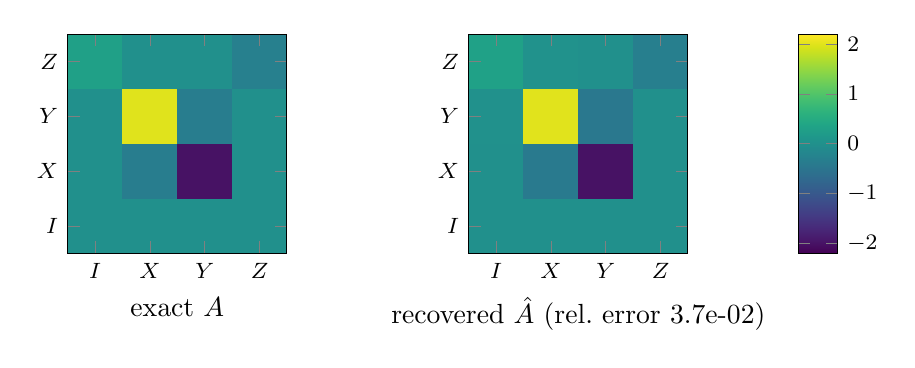
\begin{tikzpicture}[]
\begin{axis}[width=0.36\linewidth, height=0.36\linewidth, xlabel={exact $A$}, ylabel={}, colormap/viridis, enlargelimits=false, axis on top, tick label style={font=\footnotesize}, xtick={0,1,2,3}, ytick={0,1,2,3}, xticklabels={$I$,$X$,$Y$,$Z$}, yticklabels={$I$,$X$,$Y$,$Z$}, point meta min=-2.2, point meta max=2.2]
\addplot[matrix plot*, point meta=explicit, mesh/cols=4] table[meta=z] {
x y z
0 0 0
1 0 0
2 0 0
3 0 0
0 1 0
1 1 -0.35
2 1 -2
3 1 0
0 2 0
1 2 2
2 2 -0.35
3 2 0
0 3 0.3
1 3 0
2 3 0
3 3 -0.3
};
\end{axis}
\begin{scope}[xshift=0.42\linewidth]
\begin{axis}[width=0.36\linewidth, height=0.36\linewidth, xlabel={recovered $\hat A$ (rel.\ error 3.7e-02)}, ylabel={}, colormap/viridis, enlargelimits=false, axis on top, tick label style={font=\footnotesize}, colorbar, xtick={0,1,2,3}, ytick={0,1,2,3}, xticklabels={$I$,$X$,$Y$,$Z$}, yticklabels={$I$,$X$,$Y$,$Z$}, point meta min=-2.2, point meta max=2.2]
\addplot[matrix plot*, point meta=explicit, mesh/cols=4] table[meta=z] {
x y z
0 0 -1.8953e-14
1 0 1.1391e-14
2 0 -3.8038e-16
3 0 1.2707e-14
0 1 -0.0073521
1 1 -0.40361
2 1 -2.0022
3 1 0.0053175
0 2 0.0086909
1 2 2.0033
2 2 -0.43421
3 2 -0.0068988
0 3 0.30491
1 3 0.031091
2 3 -0.0024902
3 3 -0.31483
};
\end{axis}
\end{scope}
\end{tikzpicture}

\caption{Generator $\bA$ of the coherence-vector dynamics $\dot x=\bA x$ of a qubit ($\omega=2$, $\gamma_1=0.3$, $\gamma_\phi=0.2$), exact (left) and recovered by least squares from $4\times 80$ noisy time steps with $S=10^4$ shots per expectation value (right). The first row is zero (trace preservation), the first column carries the affine part $\vec\beta$ due to relaxation, the $XY$ block is the rotation at frequency $\omega$ damped at rate $\gamma_1/2+\gamma_\phi$. A toy re-computation in the spirit of the two-qubit experiments of \citet{Parvaiz2025}; generated by \texttt{code/ch11\_lindblad\_id.py}.}
\label{fig:ch11:lindblad}
\end{figure}}
\onp{\begin{center}\resizebox{0.9\linewidth}{!}{% Generated by code/ch11_lindblad_id.py -- do not edit by hand.
\definecolor{qocA}{rgb}{0.00,0.45,0.70}
\definecolor{qocB}{rgb}{0.90,0.60,0.00}
\definecolor{qocC}{rgb}{0.00,0.62,0.45}
\definecolor{qocD}{rgb}{0.80,0.40,0.00}
\definecolor{qocE}{rgb}{0.80,0.60,0.70}
\definecolor{qocF}{rgb}{0.35,0.70,0.90}
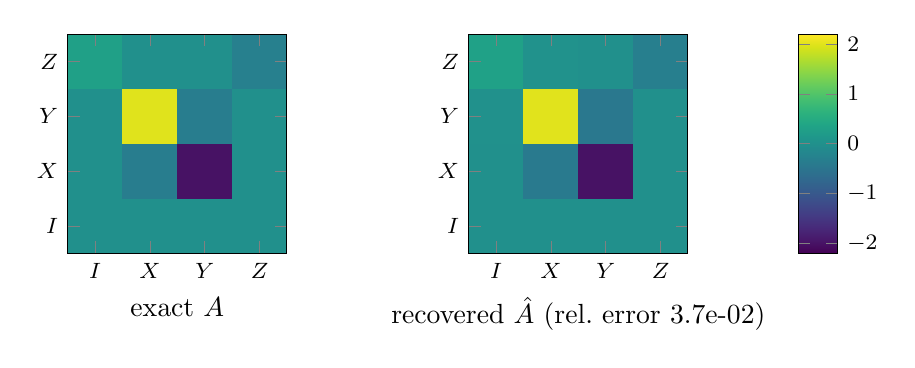
\begin{tikzpicture}[]
\begin{axis}[width=0.36\linewidth, height=0.36\linewidth, xlabel={exact $A$}, ylabel={}, colormap/viridis, enlargelimits=false, axis on top, tick label style={font=\footnotesize}, xtick={0,1,2,3}, ytick={0,1,2,3}, xticklabels={$I$,$X$,$Y$,$Z$}, yticklabels={$I$,$X$,$Y$,$Z$}, point meta min=-2.2, point meta max=2.2]
\addplot[matrix plot*, point meta=explicit, mesh/cols=4] table[meta=z] {
x y z
0 0 0
1 0 0
2 0 0
3 0 0
0 1 0
1 1 -0.35
2 1 -2
3 1 0
0 2 0
1 2 2
2 2 -0.35
3 2 0
0 3 0.3
1 3 0
2 3 0
3 3 -0.3
};
\end{axis}
\begin{scope}[xshift=0.42\linewidth]
\begin{axis}[width=0.36\linewidth, height=0.36\linewidth, xlabel={recovered $\hat A$ (rel.\ error 3.7e-02)}, ylabel={}, colormap/viridis, enlargelimits=false, axis on top, tick label style={font=\footnotesize}, colorbar, xtick={0,1,2,3}, ytick={0,1,2,3}, xticklabels={$I$,$X$,$Y$,$Z$}, yticklabels={$I$,$X$,$Y$,$Z$}, point meta min=-2.2, point meta max=2.2]
\addplot[matrix plot*, point meta=explicit, mesh/cols=4] table[meta=z] {
x y z
0 0 -1.8953e-14
1 0 1.1391e-14
2 0 -3.8038e-16
3 0 1.2707e-14
0 1 -0.0073521
1 1 -0.40361
2 1 -2.0022
3 1 0.0053175
0 2 0.0086909
1 2 2.0033
2 2 -0.43421
3 2 -0.0068988
0 3 0.30491
1 3 0.031091
2 3 -0.0024902
3 3 -0.31483
};
\end{axis}
\end{scope}
\end{tikzpicture}
}\end{center}
$\omega=2$, $\gamma_1=0.3$, $\gamma_\phi=0.2$; $4$ initial states $\times$ $80$ steps, $S=10^4$ shots per value. First column $=\vec\beta$ (relaxation), $XY$ block $=$ damped rotation.}
\end{frame}

\section{Hamiltonian identification as polynomial optimization}

\begin{frame}\ft{Hamiltonian identification via QCPOP}
\ona{The ability to write quantum control problems as polynomial optimization (\Chap~\ref{C.AlgControl}) is also useful for identification. If $H=\sum_j c_jH_j+\lambda(t)V$ has uncertain parameters $\{c_j\}$, we can find them by (i) choosing a control function $\lambda(t)$; (ii) letting the system evolve for a time $T$ and measuring the result to determine the unitary $U^\star$ it generates; (iii) minimising $\norm{U(T)-U^\star}^2$ over $\{c_j\}$, where $U(T)$ is the unitary generated by $H$. As for control, this minimisation is well approximated by a polynomial optimization problem through a truncated Magnus expansion $\Lambda_n$ of the generator. In the numerical illustration the drift is known but the interaction Hamiltonian has unknown couplings,}
\begin{equation}\label{eq:ch11:Vunknown}
     V = \begin{pmatrix} 0 & z_1 & 0 \\ z_1 & 0 & z_2 \\ 0 & z_2 & 0 \end{pmatrix},\qquad
     \min_{\mathbf{z}}\ \norm{\ee^{\Lambda_n/2}-\ee^{-\Lambda_n/2}U^\star}^2 ,
\end{equation}
\ona{a physically natural formulation: diagonal elements (eigenenergies) are easy to measure, and the zero pattern of $V$ follows from symmetry (selection rules). Driving with a known control signal $\mathbf{x}$ and performing tomography of $U^\star$, a \emph{single} pair $\mathbf{x}\to U^\star$ suffices to recover $\mathbf{z}$ with high accuracy: for 1000 random control signals, the polynomial problem with $n=3$, $p=5$ solved by TSSOS \citep{TSSOS} and refined locally recovered the couplings essentially exactly. The same reformulation shows that quantum control and identification problems, uncomputable on a Turing machine in the exact sense \citep{bondar_uncomputability_2020}, become computable in the Blum--Shub--Smale model of real computation.}
\onp{\begin{itemize}\setlength\itemsep{0.5em}
    \item Unknown $c_j$ in $H=\sum_jc_jH_j+\lambda(t)V$: drive with known $\lambda$, tomograph $U^\star$, minimise $\norm{U(T)-U^\star}^2$ over $c$.
    \item Magnus truncation $\Rightarrow$ polynomial in $c$ $\Rightarrow$ moment--SOS (TSSOS) gives the \alert{global} minimiser; one pair $\mathbf{x}\to U^\star$ suffices in the 3-level example.
    \item Mirror image of QCPOP (\Chap~\ref{C.AlgControl}): there $H$ known, controls unknown; here controls known, $H$ unknown.
    \item Side effect: computability in the BSS model \citep{bondar_uncomputability_2020}.
\end{itemize}}
\end{frame}

\begin{frame}\ft{Summary}
\begin{itemize}\setlength\itemsep{0.5em}
    \item State tomography: linear inversion is unbiased but unphysical; MLE and projected least squares enforce $\hat\rho\succeq0$; compressed sensing and classical shadows exploit low rank and locality to beat $\bigTheta{d^2}$ copies.
    \item Process tomography: standard or ancilla-assisted, CPTP enforced by a conic projection; noisy circuits become \emph{easier} to learn; gate set tomography is self-consistent up to a gauge.
    \item Open-system identification: ERA and Koopman methods realise the LDS from Hankel matrices; polynomial optimization imposes $\Gamma\succeq0$ and certifies global optimality.
    \item Reconstruction: $(\vec\theta,\vec\gamma)$ follow from $(\bA,\vec\beta)$ when $\bM$ (or $\bT_1,\bT_3$ on the physical support) has full column rank; errors are amplified by $\kappa(\bM)$.
    \item Next: the same polynomial machinery, with the roles of $H$ and $u$ exchanged, for control (\Chap~\ref{C.AlgControl}).
\end{itemize}
\end{frame}

\biblio
\end{document}
